%% LyX 2.0.1 created this file.  For more info, see http://www.lyx.org/.
%% Do not edit unless you really know what you are doing.
\documentclass[english]{article}
\usepackage[T1]{fontenc}
\usepackage[latin9]{inputenc}
\usepackage{geometry}
\geometry{verbose,tmargin=1cm,bmargin=1cm,lmargin=1in,rmargin=1in,headheight=1cm,headsep=1cm,footskip=1cm}
\pagestyle{empty}
\setcounter{secnumdepth}{2}
\setcounter{tocdepth}{2}
\usepackage{graphicx}
\usepackage{babel}
\begin{document}
\begin{center}

{\huge Daily Rook's Walk: {\huge \today}}{\huge \par}

\rule[0.5ex]{1\columnwidth}{1pt}
Rules:
\begin{enumerate}
\item row and col sums must match all numbers.
\item you must turn 90 degrees at each number.
\item numbers can't point past other numbers. 
\end{enumerate}

%%{\huge Easy}{\huge \par}

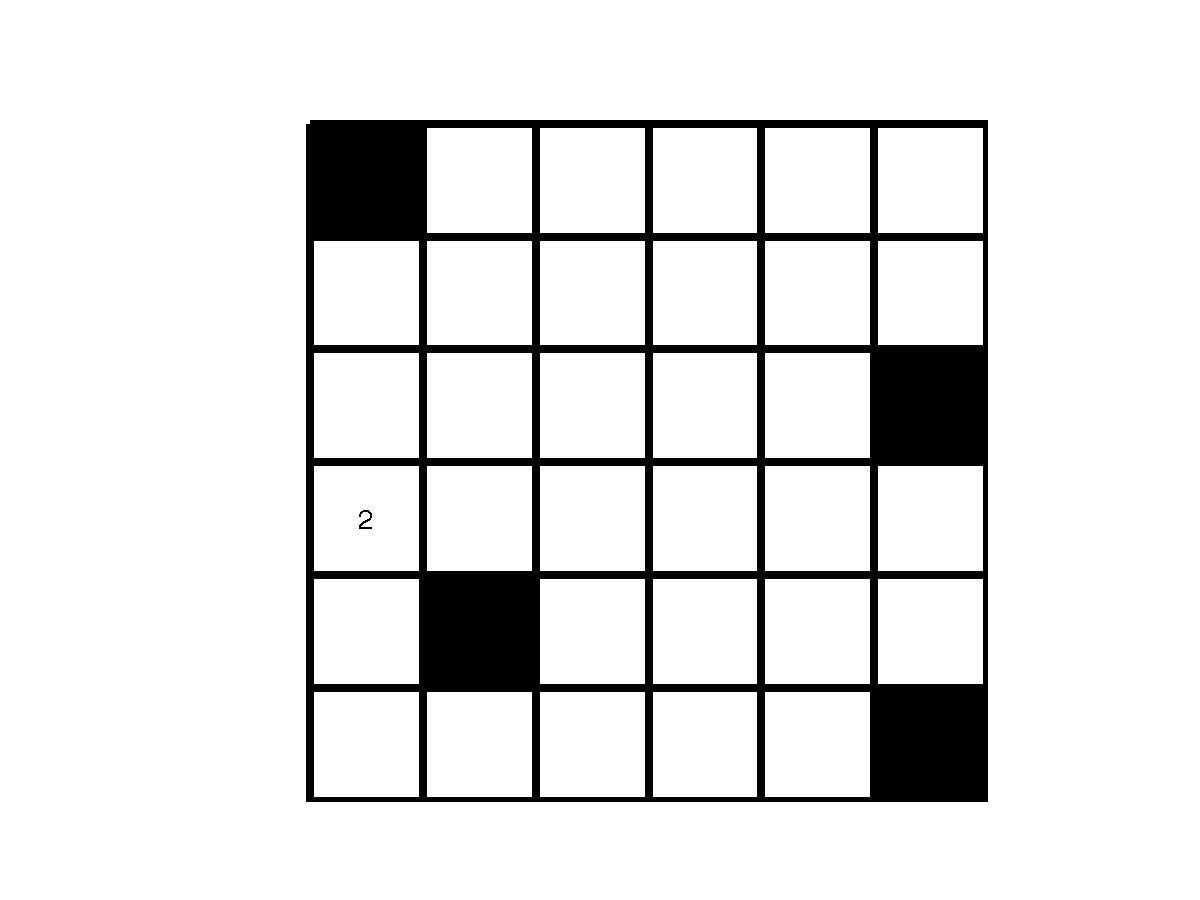
\includegraphics[scale=0.50]{easy}

%%{\huge Medium}{\huge \par}

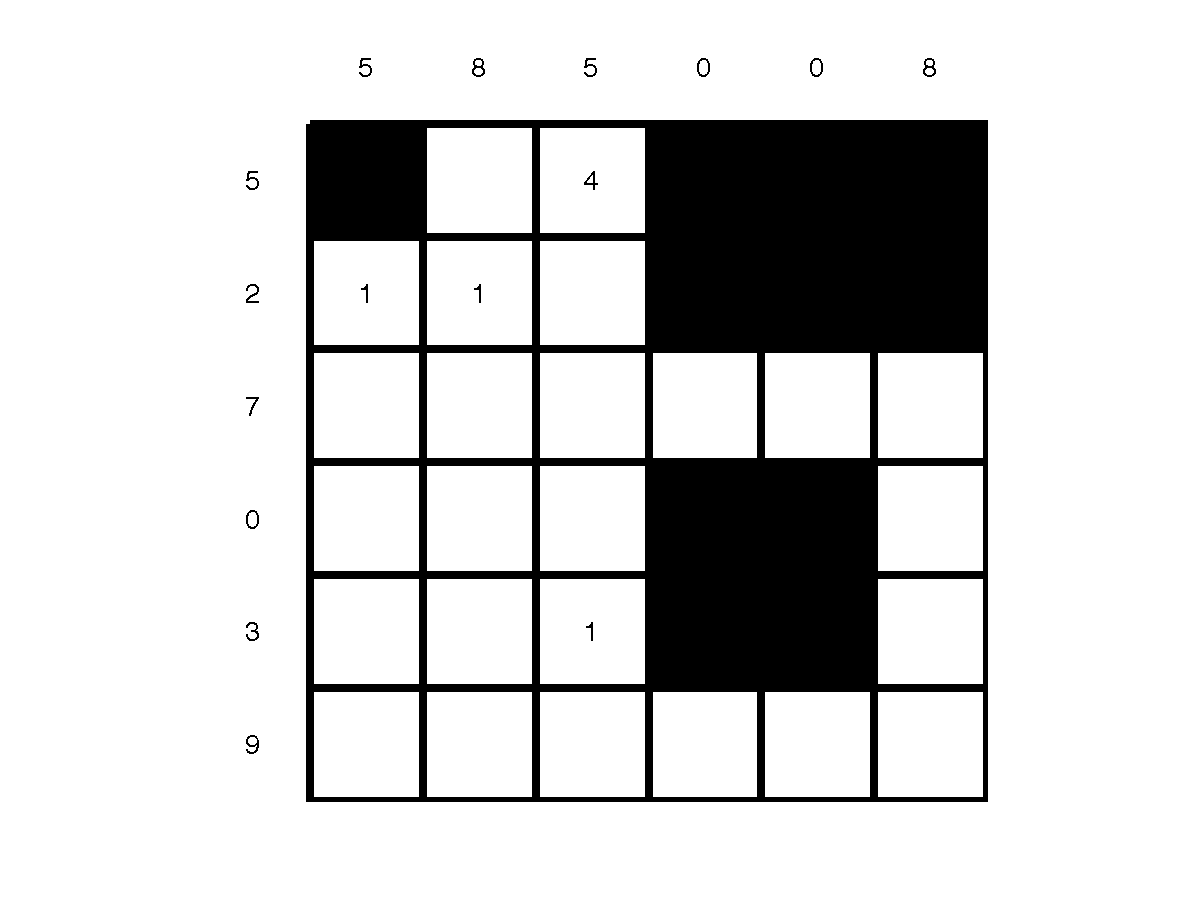
\includegraphics[scale=0.50]{medium}

\newpage
Rules:
\begin{enumerate}
\item Numbers in each row and col must be different.
\item you must turn 90 degrees at each number.
\item numbers can't point past other numbers. 
\end{enumerate}

%%{\huge Harder}{\huge \par}

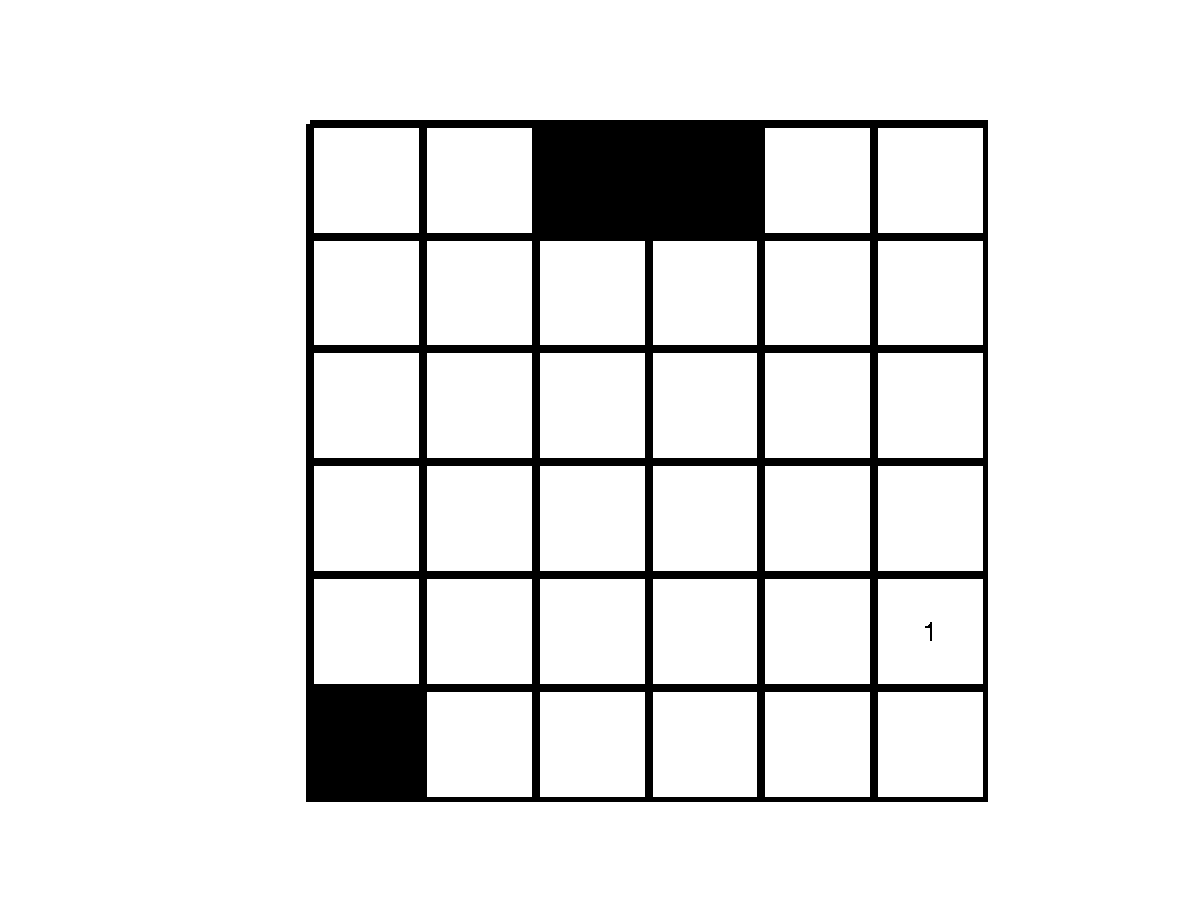
\includegraphics[scale=0.50]{harder}

%%{\huge Hardest}{\huge \par}

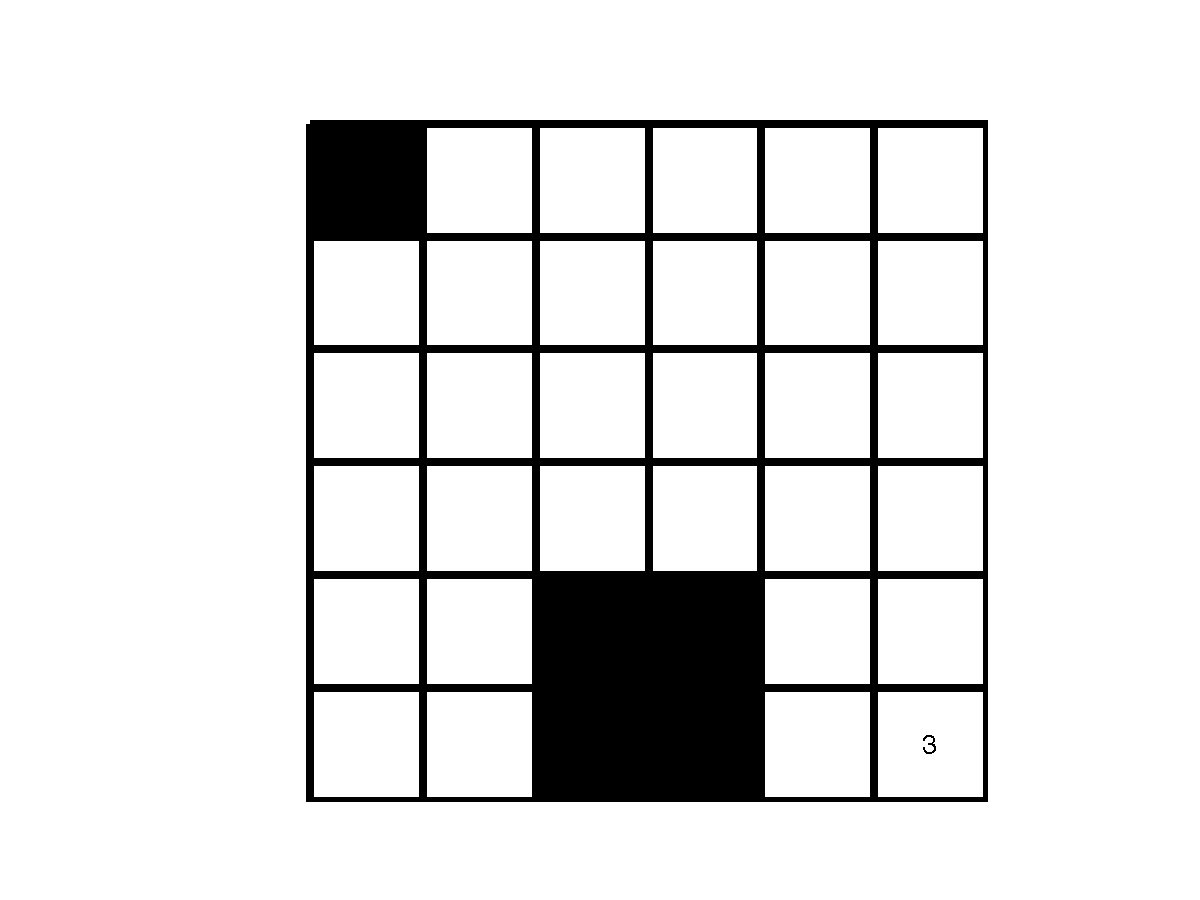
\includegraphics[scale=0.50]{hardest}

\end{center}
\end{document}
